\documentclass[11pt]{article}
\usepackage{amsmath,amsthm,amssymb,fullpage,graphicx,hyperref,listings}
\usepackage{listings,color,setspace}
\author{Andy Reagan}
\title{Math 337 Homework 05}

     \def\NN{\mathbb{N} }
     \def\ZZ{\mathbb{Z} }
     \def\QQ{\mathbb{Q} }
     \def\RR{\mathbb{R} }
     \def\CC{\mathbb{C} }
     \def\f{\frac }
     \def\b{\begin }
     \def\e{\end }
     \def\Log{\text{Log} \,}
     \def\Re{\text{Re} \, }

\lstset{language=MATLAB,
basicstyle=\ttfamily\scriptsize\singlespacing,
keywordstyle=\color{blue},
stringstyle=\color{red},
commentstyle=\color{green},
morecomment=[l][\color{magenta}]{\#},
frame=L,
xleftmargin=\parindent,
%%numbers=left,                   %% where to put the line-numbers
%%numberstyle=\scriptsize,      %% the size of the fonts that are used for the line-numbers
%%stepnumber=1,                   %% the step between two line-numbers. If it is 1 each line will be numbered
numbersep=5pt,
breaklines=true,        %% sets automatic line breaking
breakatwhitespace=false,    %% sets if automatic breaks should only happen at whitespace
escapeinside={\%*}{*)} 
}


     \newcommand{\pdiff}[2]{\frac{\partial #1}{\partial #2}}
     \newcommand{\partialdiff}[2]{\frac{\partial #1}{\partial #2}}
     \newcommand{\pdiffsq}[2]{\frac{\partial^2 #1}{{\partial #2}^2}}
     \newcommand{\pdiffcu}[2]{\frac{\partial^3 #1}{{\partial #2}^3}}
     \newcommand{\pdiffhi}[3]{\frac{\partial^#3 #1}{{\partial #2}^#3}}
     \newcommand{\diff}[2]{\frac{{\rm d}#1}{{\rm d}#2}}
     \newcommand{\diffsq}[2]{\frac{{\rm d}^{2}#1}{{\rm d} {#2}^2}}
     \newcommand{\diffhi}[3]{\frac{{\rm d}^#3 #1}{{\rm d} {#2}^#3}}
     \newcommand{\tdiff}[2]{\mbox{d} #1/\mbox{d} #2}
     \newcommand{\tdiffsq}[2]{\mbox{d}^{2} #1/\mbox{d} {#2}^2}
     \newcommand{\tpdiff}[2]{\partial #1/\partial #2}
     \newcommand{\tpdiffsq}[2]{\partial^2 #1/\partial {#2}^2}
     \newcommand{\bvec}[1]{\vec{ {\bf #1 } }}
     \newcommand{\oh}[1]{O(h^{{#1}})}

\begin{document}
\maketitle

\begin{enumerate}

\item In the three examples below, write the given higher-oder ODE(s) as a system of first-order ODEs.

\begin{enumerate}
\item The equation for the charge on the capacitor in an electric circuit:
\[ L \diffsq{Q}{t} + R \diffsq{Q}{t} + CQ = \epsilon ; \]
here $Q$ is the charge, and $L, R$ and $C$ are the inductange, resistance, and capacitance of the circuit.

\item The equation for the deflection of a loaded beam from the horizontal axis:
\[ E \f{y''}{(1+(y')^2)^{3/2}} = M(x) ; \]
here $E$ is the beam's elacticity modeulus, $Y$ is the deflection, and $M$ is the bending moment.

\item The equations of the Kepler two-body problem (5.30):
  \[ q'' = - \f{q}{(q^2+r^2)^{3/2}} ~~,~~~~~r'' = - \f{r}{(q^2+r^2)^{3/2}};  \]
where $q$ and $r$ are the cartesian coordinates of a certain radius vector relative to the center of mass of the bodies.

\end{enumerate}
\bigskip
\textbf{Solution:} 

\begin{enumerate}
\item Set $S = \tdiff{Q}{t}$ and therefore we have the system of equations
\begin{align} & L \diff{S}{t} + R \diff{S}{t} + CQ = \epsilon\\
& S = \diff{Q}{t} .\end{align}
This can be written
\begin{align} \diff{S}{t} &= \f{\epsilon - CQ}{L+R}\\
\diff{Q}{t} &= S.\end{align}

\item Set $y' = z$, such that $z' = y''$. We then have the system of ODEs
\begin{align*} y' &= z \\
z' &= \f{M(x)}{E} (1+z^2)^{3/2} \end{align*}

\item Set $q' = z$ and $r' = w$. Then we have the following system of four ODE's:
\begin{align*} z' &= -\f{q}{(q^2+r^2)^{3/2}} \\
               w' &= - \f{r}{(q^2+r^2)^{3/2}} \\
               q' &= z\\
               r' &= w.\end{align*}

\end{enumerate}

\clearpage
\pagebreak
\item Write down the explicit (i.e., component by component) equations for the (a) Midpoint method and (b) the cRK method for a system of two ODEs
$\bvec{y}' = \bvec{f} (x,\bvec{y})$.

\bigskip
\textbf{Solution:} (a) I extend the Midpoint method in a straightforward way:
\begin{align*} Y_{n+1} ^{(1)} &= Y_{n} ^{(1)} + h f ^{(1)} \left( x_n, \left\{ Y^{(1)} _n + hf ^{(1)} \left( x_n, \left\{Y^{(1)} _n , Y^{(2)} _n \right\}\right) , Y^{(2)} _n + hf ^{(2)} \left( x_n, \left\{Y^{(1)} _n , Y^{(2)} _n \right\} \right\}\right)\right)\\
Y_{n+1} ^{(2)} &= Y_{n} ^{(2)} + h f ^{(2)} \left( x_n, \left\{ Y^{(1)} _n + hf ^{(1)} \left( x_n, \left\{Y^{(1)} _n , Y^{(2)} _n \right\}\right) , Y^{(2)} _n + hf ^{(2)} \left( x_n, \left\{Y^{(1)} _n , Y^{(2)} _n \right\} \right\}\right)\right) \end{align*}

(b) The cRK coefficients become
\begin{align*} k_1 ^{(1)} &= hf^{(1)} \left (x_n, \left\{ Y^{(1)}_n, Y^{(2)}_n \right\} \right ) \\
k_1 ^{(2)} &= hf^{(2)} \left (x_n, \left\{ Y^{(1)}_n , Y^{(2)}_n \right\} \right ) \\
k_2 ^{(1)} &= hf^{(1)} \left (x_n+h/2, \left\{ Y^{(1)}_n + k_1 ^{(1)}/2, Y^{(2)}_n + k_1 ^{(2)}/2\right\} \right ) \\
k_2 ^{(2)} &= hf^{(2)} \left (x_n+h/2, \left\{ Y^{(1)}_n + k_1 ^{(1)}/2, Y^{(2)}_n + k_1 ^{(2)}/2\right\} \right) \\
k_3 ^{(1)} &= hf^{(1)} \left (x_n+h/2, \left\{ Y^{(1)}_n + k_2 ^{(1)}/2, Y^{(2)}_n + k_2 ^{(2)}/2\right\} \right ) \\
k_3 ^{(2)} &= hf^{(2)} \left (x_n+h/2, \left\{ Y^{(1)}_n + k_2 ^{(1)}/2, Y^{(2)}_n + k_2 ^{(2)}/2\right\} \right ) \\
k_4 ^{(1)} &= hf^{(1)} \left (x_n+h, \left\{ Y^{(1)}_n + k_3 ^{(1)}, Y^{(2)}_n + k_3 ^{(2)}\right\} \right ) \\
k_4 ^{(2)} &= hf^{(2)} \left (x_n+h, \left\{ Y^{(1)}_n + k_3 ^{(1)}, Y^{(2)}_n + k_3 ^{(2)}\right\} \right ) . \end{align*} 

And the next step is

\begin{align*} Y_{n+1}^{(1)} &= Y_n ^{(1)} + \f{1}{6} \left( k_1 ^{(1)} + 2k_2 ^{(1)} + 2k_3 ^{(1)} + k_4 ^{(1)} \right ) \\
Y_{n+1}^{(2)} &= Y_n ^{(2)} + \f{1}{6} \left( k_1 ^{(2)} + 2k_2 ^{(2)} + 2k_3 ^{(2)} + k_4 ^{(2)} \right ) \end{align*}

\clearpage
\pagebreak
\item 
\begin{enumerate}
\item Show that the local truncation error of the simple-central-difference method (5.12) equals
\[ \f{h^4}{12} \diffhi{y(x_n)}{x}{4} + O(h^5) .\]
Note that in the calculation of the local truncation error at the ($n$+1)st node that error at all previous nodes must be set equal to zero.

\item Show that the local truncation error of Numerov's method (5.18) equals
\[ -\f{h^6}{240} \diffhi{y(x_n)}{x}{6} + O(h^7) .\]
Hint: Note that $f_{n\pm 1} = f(x_n \pm h, y(x_n \pm h)) \equiv f[x_n \pm h ]$, where $f[x] \equiv f(x,y(x))$.
Now use the Taylor expansion for $f_{n\pm 1} $ written in the above form.
Now recall that $f = y''$.
What can you then say about $\tdiff{f}{x}$, etc?
\end{enumerate}

\bigskip
\textbf{Solution:}
\begin{enumerate}
\item The simple central difference formula is
\[ Y_{n+1} -2 Y_{n} + Y_{n-1} = h^2 f_n .\]
Since we're solving for the error, we consider $Y_n$ to be exact, hence $Y_n = y_n$.
Therefore we use Taylor expansions for the above terms as follows (bringing the $h^2f_n$ to the LHS):
\begin{align*} Y_{n+1} &:~~~~~ y_n + hy_n' + \f{h^2}{2} y_n'' + \f{h^3}{6} y_n ''' + \f{h^4}{24} y_n^{(4)} + \oh{5} \\
-2Y_{n} &:~~~~~ -2y_n\\
Y_{n-1} &:~~~~~ y_n - hy_n' + \f{h^2}{2} y_n'' - \f{h^3}{6} y_n ''' + \f{h^4}{24} y_n^{(4)} + \oh{5} \\
-h^2f_{n} &:~~~~~ -h^2y_n'' \end{align*}
Inspecting the above terms, we notice that when we add them, all of the $y_n, hy_n, h^2y_n$ and $h^3y_n$ terms cancel.
Therefore, we have the local truncation error as the remaining terms:
\[ \f{h^4}{12} y_n ^{(4)} + \oh{5} .\]

\item Numerov's formula is given similarly by
\[ Y_{n+1} -2 Y_{n} + Y_{n-1} = \f{h^2}{12} \left ( f_{n+1} + 10 f_{n} + f_{n-1} \right ).\]
Bringing everything to the LHS, we have
\[ Y_{n+1} -2 Y_{n} + Y_{n-1} -\f{h^2}{12} f_{n+1} - \f{5 h^2}{6} f_{n} -\f{h^2}{12}  f_{n-1}  = 0.\]
Since we're solving for the error, we consider $Y_n$ to be exact, hence $Y_n = y_n$.
Therefore we use Taylor expansions for the above terms as follows (bringing the $h^2f_n$ to the LHS):
\begin{align*} Y_{n+1} &:~~~~~ y_n + hy_n' + \f{h^2}{2} y_n'' + \f{h^3}{6} y_n ''' + \f{h^4}{24} y_n^{(4)} + \f{h^5}{120} y_n^{(5)} + \f{h^6}{720} y_n^{(6)} + \oh{7} \\
-2Y_{n} &:~~~~~ -2y_n\\
Y_{n-1} &:~~~~~ y_n - hy_n' + \f{h^2}{2} y_n'' - \f{h^3}{6} y_n ''' + \f{h^4}{24} y_n^{(4)} - \f{h^5}{120} y_n^{(5)} + \f{h^6}{720} y_n^{(6)} + \oh{7} \\
-\f{h^2}{12}f_{n+1} &:~~~~~ -\f{h^2}{12}y_{n+1}'' =  -\f{h^2}{12}y_n'' -\f{h^3}{12}y_n''' - \f{h^4}{24} y_n^{(4)} - \f{h^5}{72} y_n ^{(5)} - \f{h^6}{288} y_n^{(6)} + \oh{7}\\
- \f{5h^2}{6}f_{n} &:~~~~~ - \f{5h^2}{6}y_{n}''\\
-\f{h^2}{12}f_{n-1} &:~~~~~ - \f{h^2}{12}y_{n-1}'' =  -\f{h^2}{12}y_n'' +\f{h^3}{12}y_n''' - \f{h^4}{24} y_n^{(4)} +\f{h^5}{72} y_n ^{(5)} - \f{h^6}{288} y_n^{(6)} + \oh{7}\end{align*}
Since there are more terms than before, I group them by orders of $h$:
\begin{align*} \oh{0}&:~~~~y_n -2y_n + y_n = 0.\\
\oh{1}&:~~~~hy_n' - hy_n' = 0.\\
\oh{2}&:~~~~\f{h^2}{2} y_n'' + \f{h^2}{2} y_n'' -\f{h^2}{12}y_n'' -\f{5h^2}{6}y_n'' -\f{h^2}{12}y_n''= 0.\\
\oh{3}&:~~~~\f{h^3}{6} y_n''' - \f{h^3}{6} y_n''' -\f{h^3}{12}y_n''' + \f{h^3}{12}y_n'''= 0.\\
\oh{4}&:~~~~\f{h^4}{24} y_n^{(4)} + \f{h^4}{24} y_n^{(4)} - \f{h^4}{24} y_n^{(4)} - \f{h^4}{24} y_n^{(4)} = 0.\\
\oh{5}&:~~~~ \f{h^5}{120} y_n^{(5)} - \f{h^5}{120} y_n^{(5)} - \f{h^5}{72} y_n ^{(5)} + \f{h^5}{72} y_n ^{(5)}= 0\\
\oh{6}&:~~~~\f{h^6}{720} y_n^{(6)} + \f{h^6}{720} y_n^{(6)} - \f{h^6}{288} y_n^{(6)}  - \f{h^6}{288} y_n^{(6)} = -\f{h^6}{240} y_n ^{(6)}\end{align*}

Therefore, we have the local truncation error as the remaining terms:
\[ \f{h^6}{40} y_n ^{(6)} + \oh{7} .\]
\end{enumerate}

\clearpage
\pagebreak
\item Show that the Verlet method (5.27) is a second-order method.
Follow the steps of a similar derivation for the Modified Euler method, presented in Sec. 5.1.

\bigskip
\textbf{Solution:} The Verlet method is given by
\begin{align*} Y_{n+1} &=Y_{n} + h V_{n} + \f{h^2}{2} f(Y_{n} ) \\
V_{n+1} &=V_{n} + \f{h}{2} \left( f(Y_{n} ) + f(Y_{n+1} ) \right ) \end{align*}

Expanding the Taylor series of the numerical method we have
\begin{align*} Y_{n+1} &=Y_{n} + h Y_{n}' + \f{h^2}{2} Y_{n}'' \\
V_{n+1} &=V_{n} + \f{h}{2} \left( V_{n}'  + f(Y_{n} + h Y_{n}' + \f{h^2}{2} Y_{n}'') \right ) \\
&=V_{n} + \f{h}{2} \left( V_{n}'  + Y_{n}'' + h Y_{n}''' + \f{h^2}{2} Y_{n}^{(4)}) \right ) \\
&=V_{n} + \f{h}{2} \left( V_{n}'  + V_{n}' + h V_{n}'' + \f{h^2}{2} V_{n}^{(3)}) \right ) \\
&=V_{n} + h V_{n}'  +\f{ h^2 }{ 2 } V_{n}'' + \f{h^3}{4} V_{n}^{(3)}) \end{align*}
making the assumption that $V_n = Y_n'$ at the previous time step, which is standard when computing the local error, because we assume $Y_n = y_n$ (hence $V_n = v_n$).

The analytical solution for these is
\begin{align*} y_{n+1} &=y_{n} + h y_{n}' + \f{h^2}{2} y_{n}'' + \oh{3} \\
v_{n+1} &=v_{n} + h v_{n}' + \f{h^2}{2} v_{n}'' + \oh{3} \end{align*}

Comparing the above analytical and numerical solutions, we see that in both $Y$ and $V$ the Verlet method has local truncation error $\oh{3}$ making the method globally second order $(\oh{2})$.

\clearpage
\pagebreak
\item In the notes, we derived the Verlet method by first going over the half-step $[x_n, x_{n+1/2}]$ with method (5.4) and then going over the remaining half $[x_{n+1/2},x_{n+1}]$ with method (5.2).
Let us refer to the resulting Verlet method (5.27) as Verlet-1.
Use the same ideas to derive a method by reversing the order of (5.3) and (5.4) (i.e. apply (5.3) over $[x_{n},x_{n+1/2}]$ and then (5.4) over $[x_{n+1/2},x_{n+1}]$).
We will refer to this method as Verlet-2.

\bigskip
\textbf{Solution:} Reversing the order of application of the symplectic Euler steps, we have
\begin{align*} x_n ~~\to ~~ x_{n+1/2}, \text{using (5.3):} ~~~~ &Y_{n+1/2} = Y_{n} + (h/2) V_{n}\\
&V_{n+1/2} = V_n + (h/2) f(Y_{n+1/2})\\
x_{n+1/2} ~~\to ~~ x_{n+1}, \text{using (5.4):} ~~~~ &V_{n+1} = V_{n+1/2} + (h/2) f(Y_{n+1/2})\\
&Y_{n+1} = Y_{n+1/2} + (h/2) V_{n+1}\end{align*}

Adding these equations, we have
\begin{align*} V_{n+1} &= V_n + hf(Y_{n+1/2})\\
&= V_n + hf(Y_n + (h/2)V_n)\\
Y_{n+1} &= Y_n + (h/2) \cdot (V_{n} + V_{n+1})\end{align*}

\clearpage
\pagebreak
\item Consider the equations of a simple harmonic oscillator (5.25), i.e.
\[ y'' = -y, ~~~~ y(0)=0, ~~~~y'(0) = 1. \]
\begin{enumerate}
\item Write out its analytical solution (consult any ODE or Physics-I textbook).

Solve this equation numerically using the following methods:
\item Verlet-1 (or Verlet-2, the results will be similar)
\item Modified Euler (5.5)
\item cRK
\item simple central-difference (5.12) with (5.17)
\item Matlab's \verb| ode45 |

In all cases, run the simulations until $t = 1000$.
To have a fair comparison among the methods, use $h = 0.2$ for the second-order methods and $h = 0.5$ for the fourth-order ones.
For the \verb|ode45|, obtain {\em two} solutions with different values of the absolute tolerance: 0.002 and 0.003.

Your ouput should contain:\\
-phase plots of the numerical solutions (one per method);\\
-plots of the error in the Hamiltonian vs time;\\
-a table summarizing which of the methods nearly conserve the Hamiltonian and which methods do not.
\end{enumerate}

\bigskip
\textbf{Solution:}
\begin{enumerate}
\item The analytical soluton (from ODE textbook...and an obvious guess for $y'' = -y$):
\[ y(t) = \sin (t) .\]

The code that does all of the things:
\lstinputlisting[language=Matlab]{andy_hw05_prb06.m}

\item Verlet-1

\begin{figure}[h!]
  \centering
    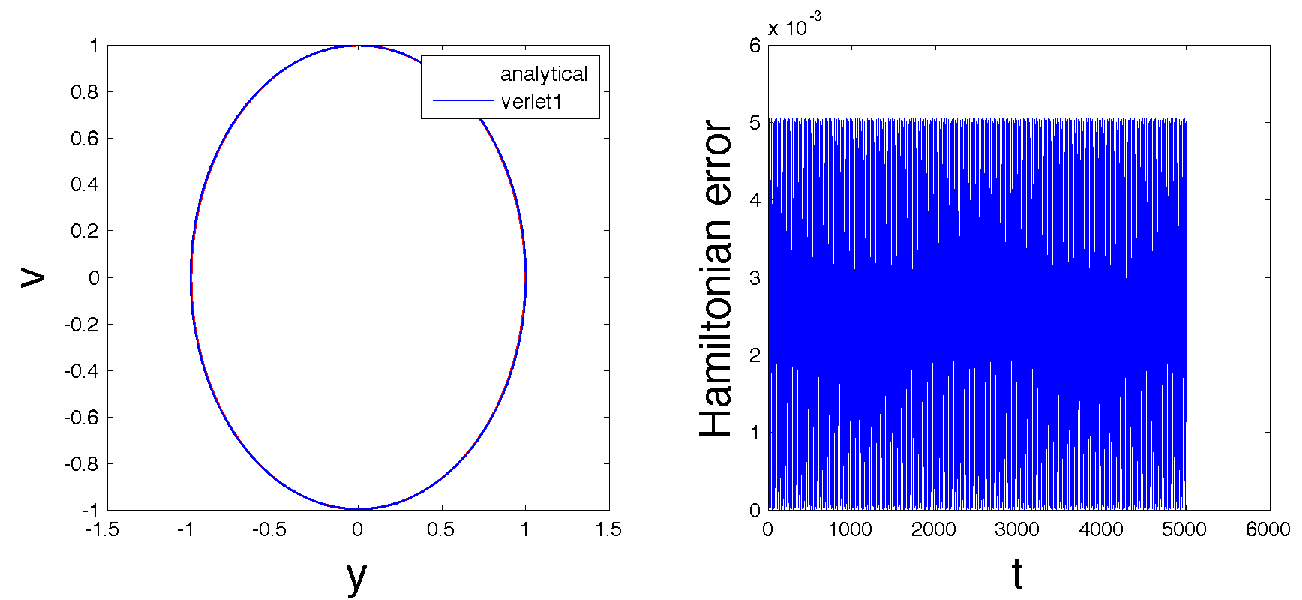
\includegraphics[width=0.9\textwidth]{andy_hw05_prb06_01.pdf}
  \caption{Harmonic oscillator solved by Verlet method.}
\end{figure}


\item Modified Euler (5.5)

\begin{figure}[h!]
  \centering
    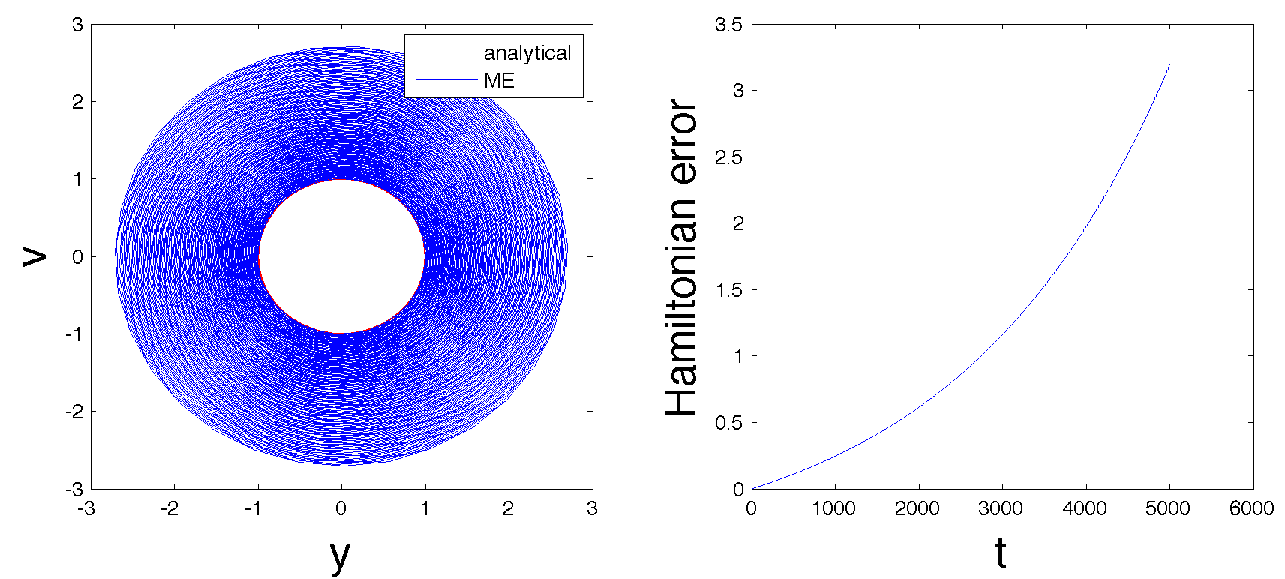
\includegraphics[width=0.9\textwidth]{andy_hw05_prb06_02.pdf}
  \caption{Harmonic oscillator solved by Modified Euler method.}
\end{figure}

\item cRK

\begin{figure}[h!]
  \centering
    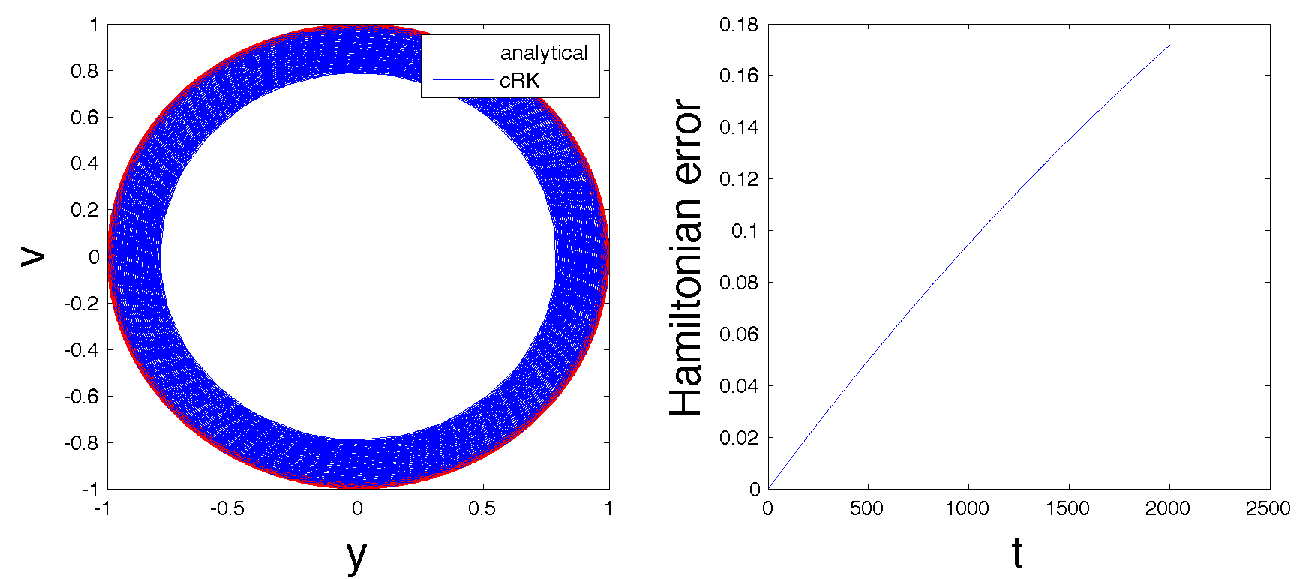
\includegraphics[width=0.9\textwidth]{andy_hw05_prb06_03.pdf}
  \caption{Harmonic oscillator solved by cRK method.}
\end{figure}

\item simple central-difference (5.12) with (5.17)

\begin{figure}[h!]
  \centering
    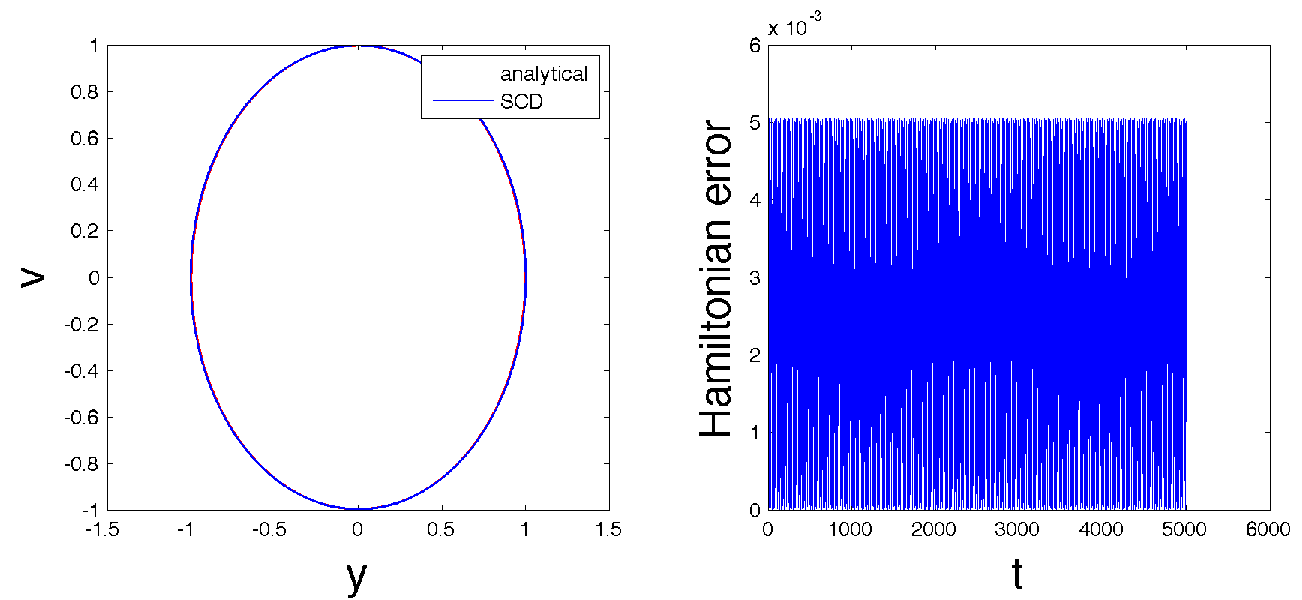
\includegraphics[width=0.9\textwidth]{andy_hw05_prb06_04.pdf}
  \caption{Harmonic oscillator solved by simple-central-difference method.}
\end{figure}

\item Matlab's \verb| ode45 |

\begin{figure}[h!]
  \centering
    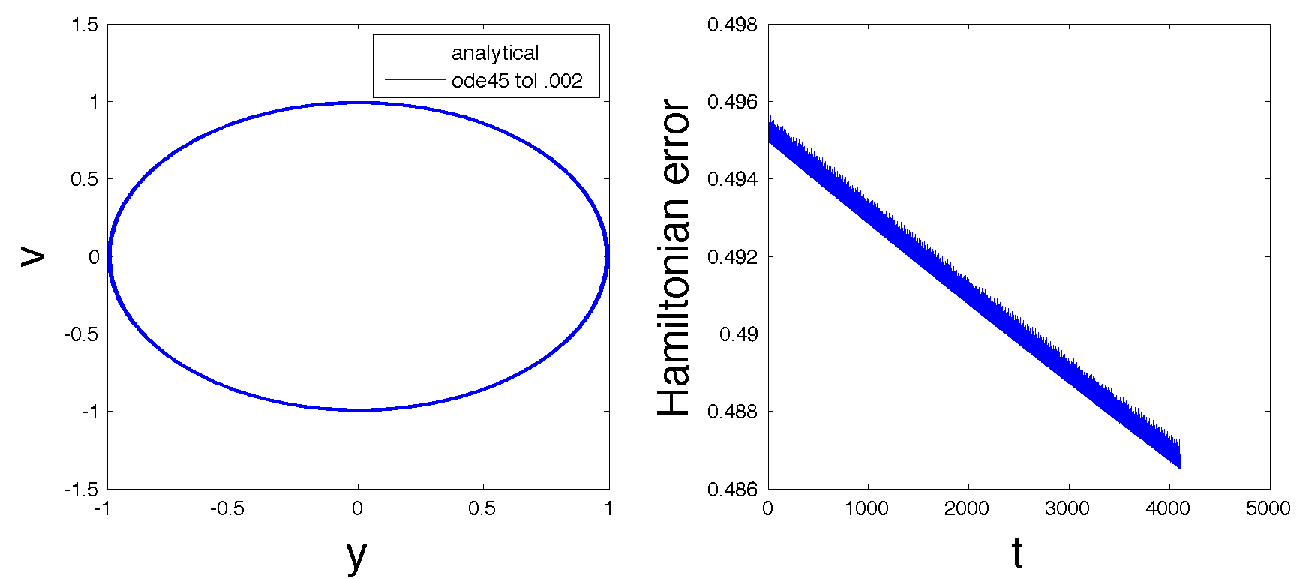
\includegraphics[width=0.9\textwidth]{andy_hw05_prb06_05.pdf}
  \caption{Harmonic oscillator solved by ode45 with tolerance .002.}
\end{figure}

\begin{figure}[h!]
  \centering
    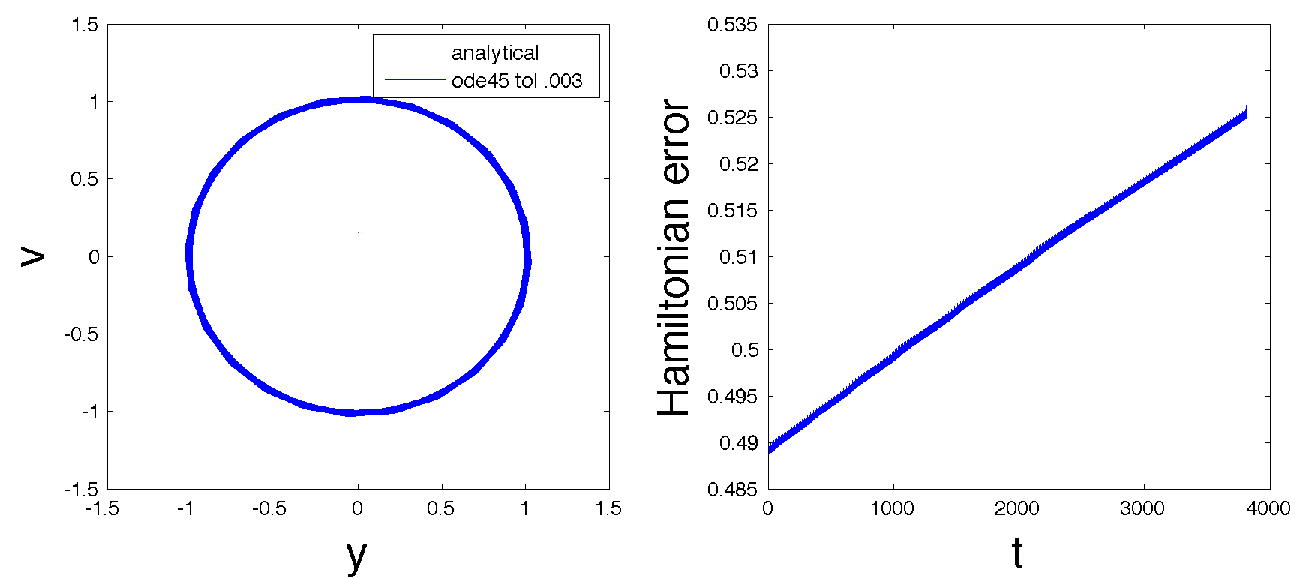
\includegraphics[width=0.9\textwidth]{andy_hw05_prb06_06.pdf}
  \caption{Harmonic oscillator solved by ode45 with tolerance .003.}
\end{figure}

Table summarizing which of the methods nearly conserve the Hamiltonian and which methods do not:


\begin{table}
\centering
\begin{tabular}[h!]{cc}
\hline
method which DO & methods which DO NOT\\
\hline
\hline
Verlet method & Modified Euler\\
simple-central-difference & cRK\\
\verb|ode45| with tolerance .002 & \verb|ode45| with tolerance .003 \\
\hline

\end{tabular}

\caption{Table summarizing which of the methods nearly conserve the Hamiltonian and which methods do not.}
\end{table}

\end{enumerate}

\clearpage
\pagebreak
\item Find an {\em estimate} for the growth of the Hamiltonian, $H = (1/2) (v^2 + y^2)$, of the numerical solution of the harmonic oscillator model obtained with the regular Euler method.
Follow the steps described below.

\begin{enumerate}
\item For concreteness, consider the IVP of Problem 6, for which you obtained the analytical solution.
Use the reult of Problem 6(a) to find the exact value of the Hamiltonian.

\item Write down the formulae for the corresponding numerical solutions obtained with the regular Euler method.
These formulae are described, but not explicitly stated, in the paragraph (including the footnote) after (5.54).
Then, with these solutions, calculate an estimate for the numerically computed Hamiltonian.

\item Finally, verify that your answer for $H_\text{computed} - H_\text{exact}$ agrees with that found from a figure in Sec. 5.3 (for the largest value of $x$).

\end{enumerate}

\bigskip
\textbf{Solution:}

\begin{enumerate}
\item From problem 6(a), we have the solution $y(t) = \sin (t)$.
Thus we have $v(t) = \cos (t)$ and can compute the Hamiltonian as
\[ H = 1/2 (\sin ^2 t + \cos^2 t) = 1/2 .\]

\item With the ODE written as a system, we have $y' = v$ and $v' = -y$. Regular Euler computes
\begin{align*} Y_{i+1} &= Y_i + h V_i\\
V_{i+1} &= V_i - h Y_i\end{align*}
Creativity being discouraged, I find the following to be a very straight forward approach.
Thus, explicitly computing that $H_0 = 1/2 \cdot( 1^2+0^2) = 1/2$, and setting $x_0 = 0$:
\begin{align*} H_{n+1} &= \f{1}{2} \left ( Y_{n+1}^2 + V_{n+1} ^2 \right )\\
&= \f{1}{2} \left ( (Y_n + h V_n)^2 + (V_n - h Y_n) ^2 \right )\\
&= \f{1}{2} \left ( (1+h^2) Y_n^2 + (1+h^2) V_n^2 \right )\\
&= \f{1}{2} (1+h^2) \left ( Y_n^2 + V_n^2 \right )\\
&= \f{1}{2} (1+h^2) 2 H_n\\
&= (1+h^2) H_n\\
&= (1+h^2)^n H_0\\
&= \f{1}{2} (1+h^2)^{(x-x_0)/h} \\
&= \f{1}{2} e^{xh} \end{align*}

\item The figure in Sec. 5.3 has  $H_\text{computed} - H_\text{exact} \approx 0.25$ for $x = 20$.
Assuming a step size of 0.02 as in the notes, we have 
\begin{align*} H_{\text{computed}} &= \f{1}{2} e^{20\cdot .02} \\
&= 0.74\end{align*}
which agress with the error of about 0.25.
This is verified in MATLAB with\\
 \verb|h = .02; 0.5*(h^2+1)^(20/h)|.

\end{enumerate}






\clearpage
\pagebreak
\item In the notes, we showed that the symplectic Euler methods (5.3) and (5.4) approximate very well the energy of a system without friction-like forces.
Now, investigate the question of whether these methods still produce accurate approximations to the energy when a small friction {\em is} present.

Consider a slightly damped harmonic oscillator
\[ y'' = -2 \gamma y' - \omega _0 ^2 y, ~~~~~y(0) = 0, ~~~~~y'(0) = 1.\]

Its exact solution is $y = \f{1}{\omega} e ^{-\gamma t} \sin (\omega t)$, where $\omega = \sqrt{\omega _0 ^2 - \gamma ^2}$.
Note that the energy of a damped oscillator is defined by the same expression as in the undamped case:
\[ E = \f{1}{2} \left ( (y')^2 + \omega _0 ^2 y ^2 \right ).\]
One can obtain the using exact solution
\[ E_\text{exact} = \f{e^{-2\gamma t}}{2\omega ^2}\left ( \omega _0 ^2 - \gamma ^2 \cos (2\omega t) - \omega \gamma \sin (2 \omega t) \right ) ~~\approx~~ \f{1}{2} e^{-2\gamma t}. \]

Use the regular Euler and one of the two symplectic Euler methods to simulate the damped oscillator with $\omega _0 = 1$ and $\gamma = 0.015$ up to $t = 50$.
For each of the methods, use three different value of step size: $h \in [0.01,0.03,0.05]$.
For each of the above values of $h$, you need to present three plots.
Plot 1 should contian the phase plane plots of the exact solution and the solution obtained by the regular Euler method.
Plot 2 should contain the phase plane plots of the exact solution and the solution obtained by the symplectic Euler method.
Plot 3 should contain the the error in the total energy for both methods.

Using an analysis similar to that you did in Problem 7, {\em explain quantitatively} why the regular Euler solution behaves, relative to the exact solution, in the observed way.
That is, give a quantitative estimate of the error in the oscillator's total energy for each given $h$ and compare it with the value you obtain from you code.
{\em Also}, you must explain why the regular Euler solution changes from decaying to growing as $h$ is varied.

Conclude whether is it reasonable to use symplectic methods for problems with {\em small} friction (or any other source of damping).
Is it a good idea to use general-purpose methods (like the regular Euler) for the same task?

\bigskip
\textbf{Solution:} The code and plots follow this discussion.

I derive why regular Euler solution behaves the way it does, and how that depends on $h$.
With the analytical solution given as in the problem statement, we compute the derivative for the analytical $v$ and we have
\[ y = \f{1}{\omega} e ^{-\gamma t} \sin (\omega t) ~~~~\Rightarrow y' = v = \f{-\gamma}{\omega} e ^{-\gamma t} \sin (\omega t) + e ^{-\gamma t} \cos (\omega t) .\]
From the notes, we know that the regular Euler solution behaves as $ye^{th/2}$ in $y$ and $ve^{th/2}$ in $v$.
Therefore, we compute the numerical total energy as (noting that $\omega_0 / \omega \approx 1$ since $\gamma$ is small):
\begin{align*} E_{\text{computed}} &= \f{1}{2} \left ( (ye^{th/2})^2 \omega _0 ^2 + (ve^{th/2}) ^2  \right ) \\
&= \f{1}{2} \left ( (\f{1}{\omega} e ^{(h/2-\gamma) t} \sin (\omega t) )^2 \omega _0 ^2 + (\f{-\gamma}{\omega} e ^{(h/2-\gamma) t} \sin (\omega t) + e ^{(h/2-\gamma) t} \cos (\omega t)) ^2  \right ) \\
&\simeq \f{1}{2} \left ( e ^{(h-2\gamma) t} \sin ^2(\omega t) - \f{\gamma^2}{\omega^2} e ^{(h-2\gamma) t} \sin^2 (\omega t) + e ^{(h-2\gamma) t} \cos^2 (\omega t)  -\f{2\gamma}{\omega} e ^{(h-2\gamma) t} \sin^2 (\omega t) \cos^2 (\omega t) \right ) \\
&= \f{1}{2}  e ^{(h-2\gamma) t} \left ( \sin ^2(\omega t) - \f{\gamma^2}{\omega^2} \sin^2 (\omega t) + \cos^2 (\omega t)  -\f{2\gamma}{\omega} \sin^2 (\omega t) \cos^2 (\omega t) \right ) \\
&\approx \f{1}{2}  e ^{(h-2\gamma) t} \end{align*}

It can be seen from the problem statement that the exact solution's total energy decays as $t$ increases.
However, we observe that the numerical solution from simple Euler decays is $h<2\gamma$, is approximately constant for $h = 2\gamma$, and grows for $h > 2\gamma$.
Since we set $\gamma = 0.015$, we have $2\gamma = 0.03$.
So for $h = 0.01$, the computed energy decays, for $h = 0.03$ the computed energy is constant, and for $h = 0.05$ the computed energy grows.
This is exactly what we observe.

It is reasonable to use symplectic methods for small friction.
However, the general purpose methods are not appropriate for this task.

\lstinputlisting[language=Matlab]{andy_hw05_prb08.m}

\begin{figure}[h!]
  \centering
    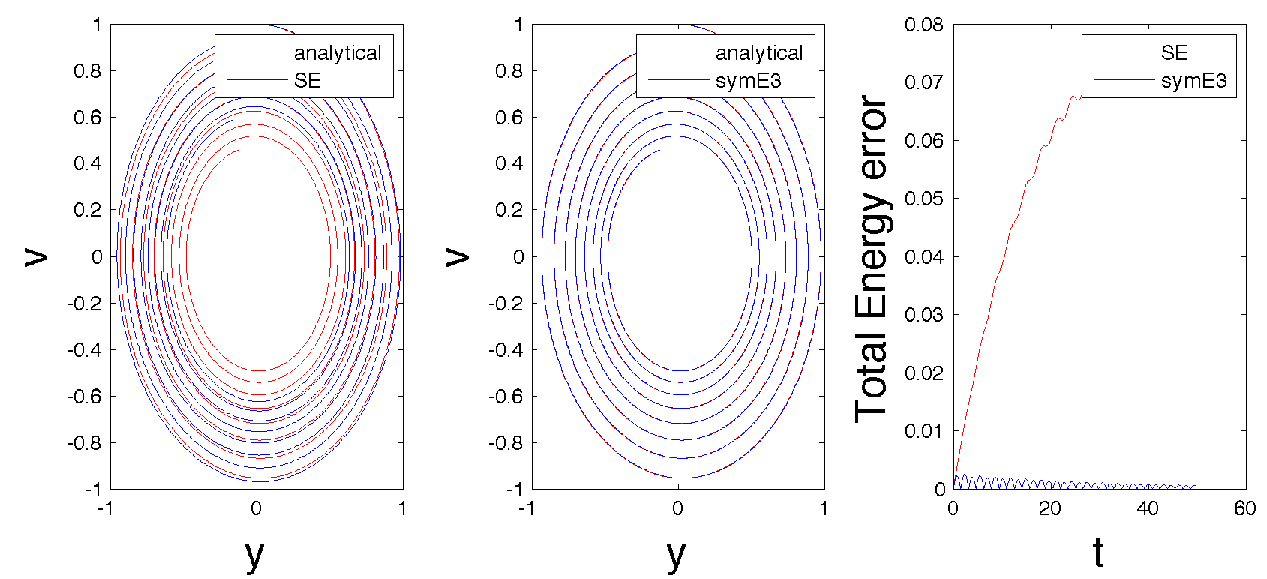
\includegraphics[width=0.9\textwidth]{andy_hw05_prb08_01.pdf}
  \caption{The simple Euler (SE) and symplectic Euler (symE3) solutions for a damped oscillator, along with the error in the total energy. The time step $h$ is set to 0.01.}
\end{figure}

\begin{figure}[h!]
  \centering
    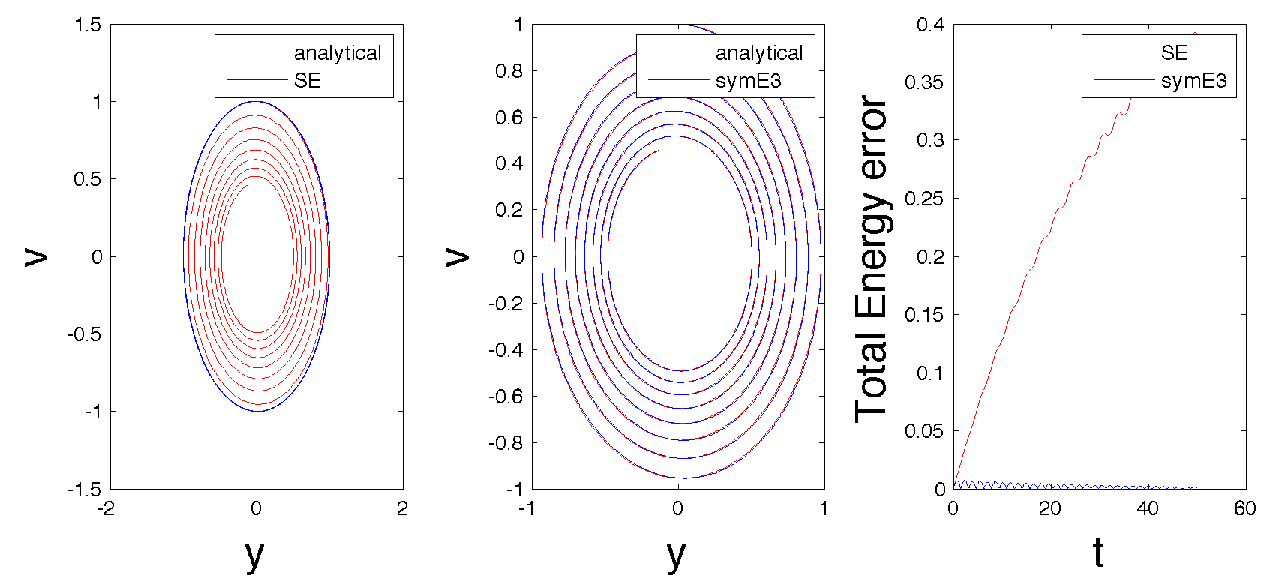
\includegraphics[width=0.9\textwidth]{andy_hw05_prb08_03.pdf}
  \caption{The simple Euler (SE) and symplectic Euler (symE3) solutions for a damped oscillator, along with the error in the total energy. The time step $h$ is set to 0.03.}
\end{figure}

\begin{figure}[h!]
  \centering
    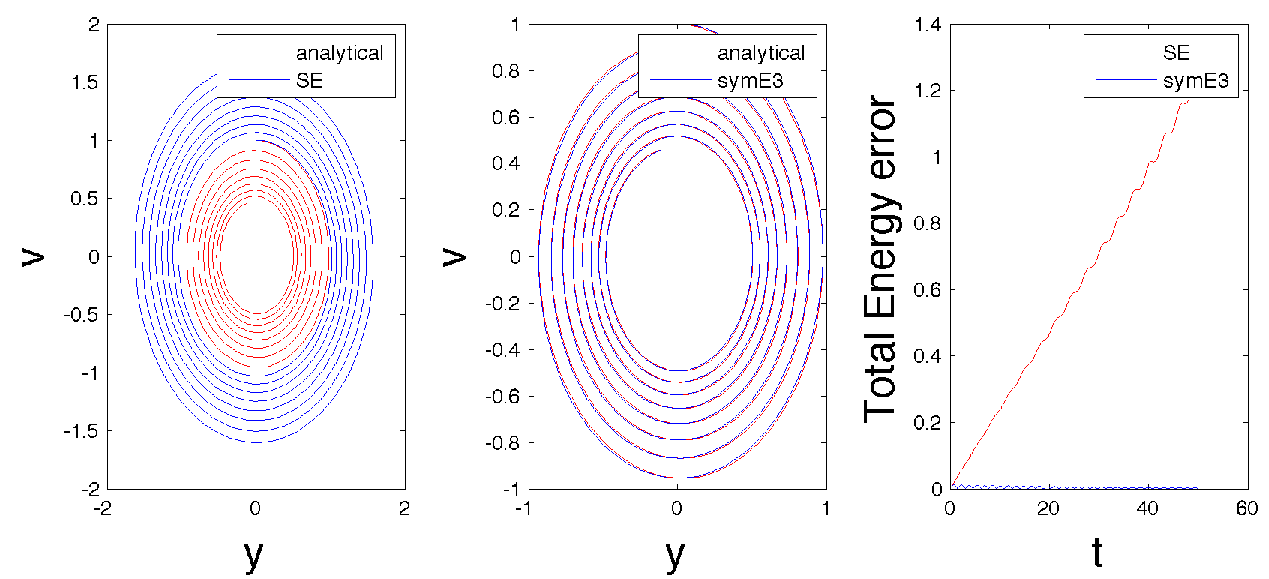
\includegraphics[width=0.9\textwidth]{andy_hw05_prb08_05.pdf}
  \caption{The simple Euler (SE) and symplectic Euler (symE3) solutions for a damped oscillator, along with the error in the total energy. The time step $h$ is set to 0.05.}
\end{figure}


\clearpage
\pagebreak
\item Follow the lines of the stability analyses for the regular and symplectic Euler methods (see Sec 5.4) and obtain the stability regions for the Modified Euler (5.5) and Verlet Method (5.27).
Use (5.25a) as the model problem for both methods, where you should assume that $\omega$ is complex (as you did earlier for $\lambda$).

Strictly speaking, you should be able to give the answers for both methods without doing any calculations, because these answers can be found in Lectures 4 and 5.
However, I would like you to do those calculations in order to get some practice with stability analysis of a system of ODEs.

\bigskip
\textbf{Solution:} For the Modified Euler method, a general purpose method, we consider the 1-D case:
\[ y' = \lambda y ,~~~~~\text{with} ~~~~\lambda = \pm i \omega .\]
Plugging this into the Modified Euler method, we have 
\begin{align*} Y_{n+1} &= Y_n \left [ 1 + h \lambda + \f{1}{2} (h\lambda )^2 \right ] \end{align*}
where $\lambda = \lambda _R + i \lambda _I$ as a complex number.
For this method to be stable, we require that the magnitude of the bracketed RHS.
This becomes
\begin{align*} & \left |1 + h \lambda + \f{1}{2} (h\lambda )^2 \right |\\
= & \left |1 + h \lambda_R + ih \lambda_I + \f{1}{2} (h \lambda_R + ih \lambda_I )^2 \right |\\
= & \sqrt{ (h \lambda_I)^2 + \left (1- \f{1}{2} h^2 \lambda_I ^2 \right) }\\
= & \sqrt{ 1+ \f{1}{4} h^4 } \\
\approx & 1 + \f{1}{8} h^4\end{align*}
Since this last approximation is the error growth at each timestep, we see that for any $h$ it is greater than 1.
Therefore any error will grow exponentially and the Modified Euler method is {\em unstable} for any $h$.

For the Verlet method:
\begin{align*} Y_{n+1} &= Y_n + hV_n + \f{h^2}{2} f(Y_n) \\
V_{n+1} &= V_n + \f{h}{2} \left ( f( Y_n) + f( Y_{n+1})\right )  \end{align*}
we use the model problem
\[ \left ( \begin{array}{c}  \omega y \\ v  \end{array} \right ) ' = \left ( \begin{array}{cc}  0 & \omega \\ -\omega & 0   \end{array} \right ) \left ( \begin{array}{c}  \omega y \\ v   \end{array} \right ). \]
Applying this problem to the Verlet method, we have the folowing system:
\[ \left ( \begin{array}{cc}  1 & 0 \\ \f{\omega ^2 h}{2} & 1 \end{array} \right ) \left ( \begin{array}{c}  \omega Y \\ V \end{array} \right )_{n+1} ' = \left ( \begin{array}{cc}  1 - \f{\omega ^2 h^2}{2} & h \\ -\f{h\omega^2}{2} & 1 \end{array} \right ) \left ( \begin{array}{c} \omega Y \\ V \end{array} \right ) _n. \]
To solve this system, we multiply on the left by the inverse of the matrix on the LHS:
\[  \left ( \begin{array}{c}  \omega Y \\ V \end{array} \right )_{n+1} ' = \left ( \begin{array}{cc}  1 & 0 \\ \f{\omega ^2 h}{2} & 1 \end{array} \right ) ^{-1} \left ( \begin{array}{cc}  1 - \f{\omega ^2 h^2}{2} & h \\ -\f{h\omega^2}{2} & 1 \end{array} \right ) \left ( \begin{array}{c} \omega Y \\ V \end{array} \right ) _n. \]
%% I solve for the inverse as
%% \[ \left ( \begin{array}{cc}  1 & 0 \\ \f{\omega ^2 h}{2} & 1 \end{array} \right ) \left ( \begin{array}{cc} a & b \\ c & d \end{array} \right ) = \left ( \begin{array}{cc} 1 & 0 \\ 0 & 1 \end{array} \right ) \]
%% and determine
We have the inverse on the RHS as
\[ \left ( \begin{array}{cc}  1 & 0 \\ \f{\omega ^2 h}{2} & 1 \end{array} \right ) ^{-1} = \left ( \begin{array}{cc}  1 & 0 \\ - \f{\omega ^2 h}{2} & 1 \end{array} \right ). \]
And so the system becomes
\begin{align*}  \left ( \begin{array}{c}  \omega Y \\ V \end{array} \right )_{n+1} ' = \left ( \begin{array}{cc}  1 - \f{\omega ^2 h^2}{2} & h \\ \f{\omega ^4 h^3}{4} -\omega ^2 h & 1 - \f{\omega ^2 h^2}{2} \end{array} \right )  \left ( \begin{array}{c} \omega Y \\ V \end{array} \right ) _n. \end{align*}
We solve for the Eigenvalues of the matrix on the RHS as
\begin{align*} & \left ( 1 - \f{\omega ^2 h^2 }{2} - \lambda \right ) \left ( - \f{\omega ^2 h^2 }{2} + 1 - \lambda \right ) - (h) \left ( -\omega ^2 h + \f{\omega ^4 h ^3 }{4} \right ) \\
&= \lambda^2 + (\omega ^2 h^2 - 2) \lambda +1 \end{align*}
We obtain
\[ \lambda_{1,2} = \f{1}{2} \left [  2 - \omega ^2 h ^2 \pm \omega h \sqrt{\omega^2 h^2 - 4} \right ] \]
and setting $z = h \omega$
\[ \lambda_{1,2} = \f{1}{2} \left [  2 - z^2 \pm z \sqrt{z ^2 - 4} \right ] .\]
I plot the boundary of this stability region in MATLAB:

\lstinputlisting[language=Matlab]{andy_hw05_prb09.m}

\begin{figure}[h!]
  \centering
    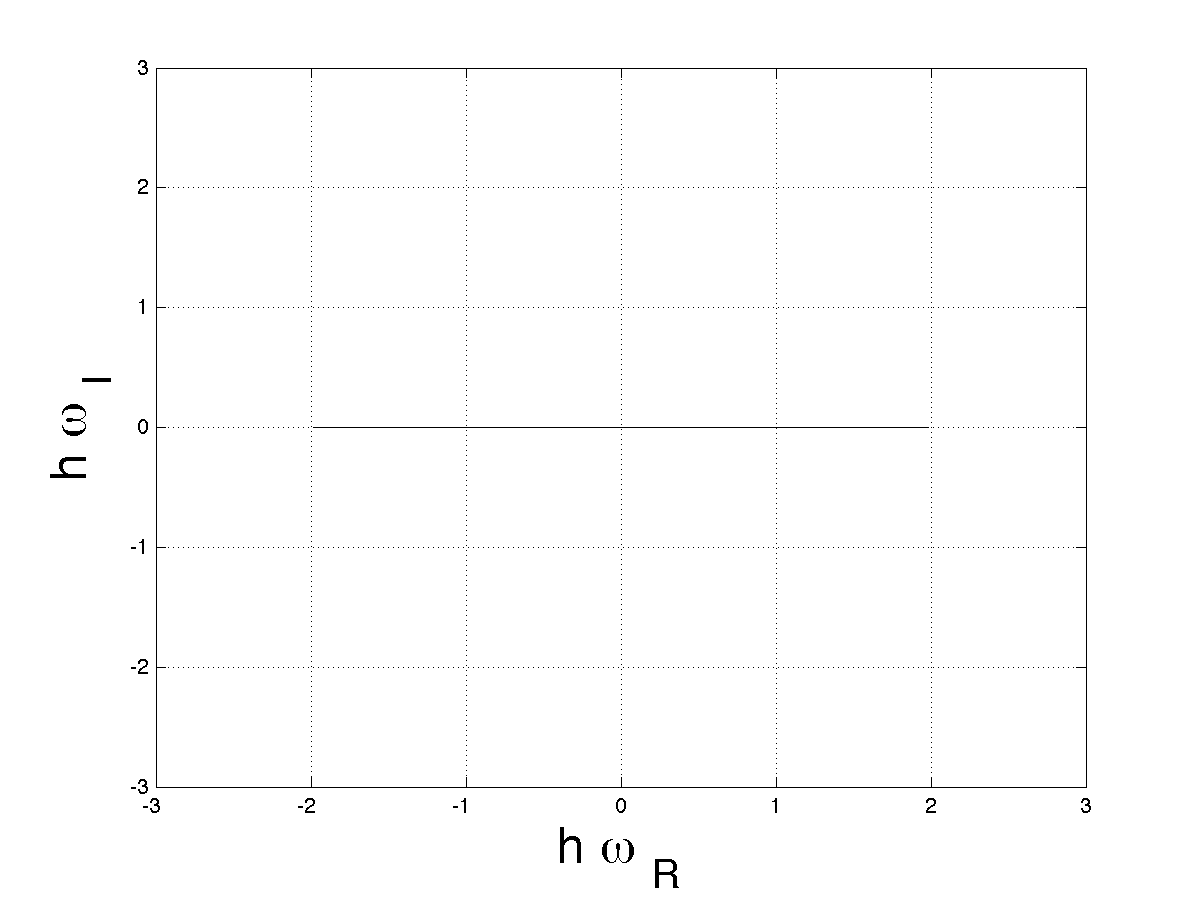
\includegraphics[width=0.5\textwidth]{andy_hw05_prb09_02.png}
  \caption{The stability region of the Verlet method.}
\end{figure}


\clearpage
\pagebreak
\item Consider a system of two linear ODEs:
\[ \diff{}{t} \left ( \begin{array}{c} x(t)\\ y(t)\end{array} \right ) = A \left ( \begin{array}{c} x(t)\\ y(t)\end{array} \right ), ~~~~~~~~~~~~~A = \left ( \begin{array}{cc} 100 & 99\\ 99 & 100\end{array} \right ). \]

\begin{enumerate}
\item Would you call this system numerically stiff?
\item Will you answer change if both entries of $A$ with 100 are replaced with -100?
Please explain.
\end{enumerate}

\bigskip
\textbf{Solution:}

\begin{enumerate}
\item No. I compute the eigenvalues of $A$:
\begin{align*} \left | \begin{array}{cc} 100 -\lambda & 99\\ 99 & 100 - \lambda \end{array} \right | &= \lambda ^2 - 200 \lambda + 100\cdot 100 - 99 \cdot 99\\
&= \lambda ^2 - 200 \lambda +199 = (\lambda -1)(\lambda -199)\end{align*}
which are thus $1,199$.
The ratio of these is large (satisfies criterion I), but the larger eigenvalue has positive real part (fails criterion II).

\item Yes. Again I compute the eigenvalues
\begin{align*} \left | \begin{array}{cc} -100 -\lambda & 99\\ 99 & -100 - \lambda \end{array} \right | &= \lambda ^2 + 200 \lambda + 100\cdot 100 - 99 \cdot 99\\
&= \lambda ^2 + 200 \lambda +199 = (\lambda +1)(\lambda + 199)\end{align*}
which are thus $-1,-199$.
The ratio of these is large (satisfies criterion I), and the larger eigenvalue has negative real part (satisfies criterion II).

\end{enumerate}




\clearpage
\pagebreak
\item[Bonus-1] Explain why the solutions of \verb|ode45| with rather similar tolerances behave {\em qualitatively} differently.

{\em Hint:} Look at the plot of its stability region. You can obtain it as in HW 4, while using the fact that \verb|ode45| employs a 5th-order accurate Runge-Kutta method to compute its solution. (To see how the last piece of information determines the stability region, review what equation(s) determined the stability regions of other Runge-Kutta type methods.)

You explanation must be sufficiently detailed and coherent to recieve credit. If you are not sure what ``sufficient'' is in this case, ask the instructor.


\bigskip
\textbf{Solution:}  Looking back at the results of Problem 6, note that \verb|ode45| used $h \simeq 0.24$ for \verb|AbsTol| $=.002$ and $h \simeq 0.26$ for \verb|AbsTol| $=.003$.
The stable region for the 5th-order RK method, as for the 4-th order in HW 4 and in the notes (remark after Eq 4.21), we expect to be the 5-th degree polynomial approximating the exact solution.
Since RK is a general-purpose method, we study the stable region as in the 1D case, setting $\lambda  = \pm i \omega$.
Specifically the 5-th order method is stable when
\begin{equation} \left | \sum _{k=0} ^5 \f{(h\lambda) ^k}{k!} \right | \leq 1 .\end{equation}

I wasn't able to to explain why the different tolerance led to such different solutions, since it seems to me that both values of $h$ are within the stability region of the 5th order method.
Here is the code, and plot, anyway:

\lstinputlisting[language=Matlab]{andy_hw05_prb11.m}

\begin{figure}[h!]
  \centering
    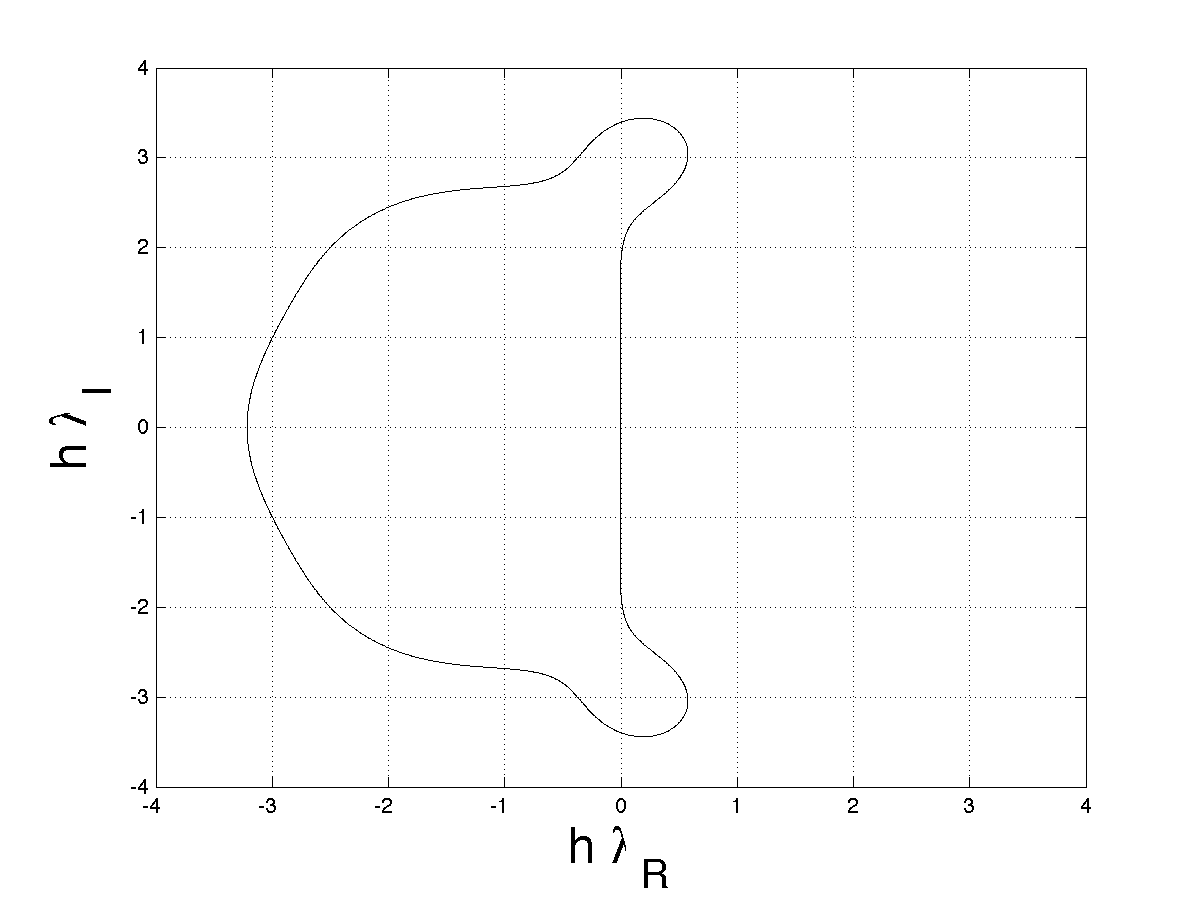
\includegraphics[width=0.5\textwidth]{andy_hw05_prb11_01.png}
  \caption{The stability region of the 5th order RK method.}
\end{figure}



\clearpage
\pagebreak
\item[Bonus-2] Apply the Verlet-1 and -2 methods to the Kepler two-body problem (5.30) (see also Problem 1(c) above). Use $h = 0.1$ and $t_{\max} =  500$. As the initial condition, use
\[ q(0) = 1-\text{ecc}, ~~~r(0) = 0,~~~Q(0) = 0, ~~~ R(0) = \sqrt{\f{1+\text{ecc}}{1-\text{ecc}}} ~~~\text{for}~ \text{ecc} = 0.6,\]
which corresponds to the exact solution being an elipse with eccentricity 0.6.
Compute the conserved quantities: the Hamiltonian (5.31), the angular momentum (5.32), and the components of the Runge-Lenz vector (5.33), and the plot them versus time.

Now plot the trajectory defined by Eqs. (5.30).
What effect does the nonconservation of the Runge-Lenz vector appear to have on the numerical solution of (5.30)?
If you are not sure, reduce the step size (but keep $t_{\max}$ the same) and see what this does to your numerical solution.

\bigskip
\textbf{Solution:} I present my code and the requested plots below.
Non-conservation of the Runge-Lenz vector causes the solution's orbit to lose orientation, in such a way that the orientation of the elipse moves entirely around the center by $t = 1000$.

\lstinputlisting[language=Matlab]{andy_hw05_prb12.m}

\begin{figure}[h!]
  \centering
    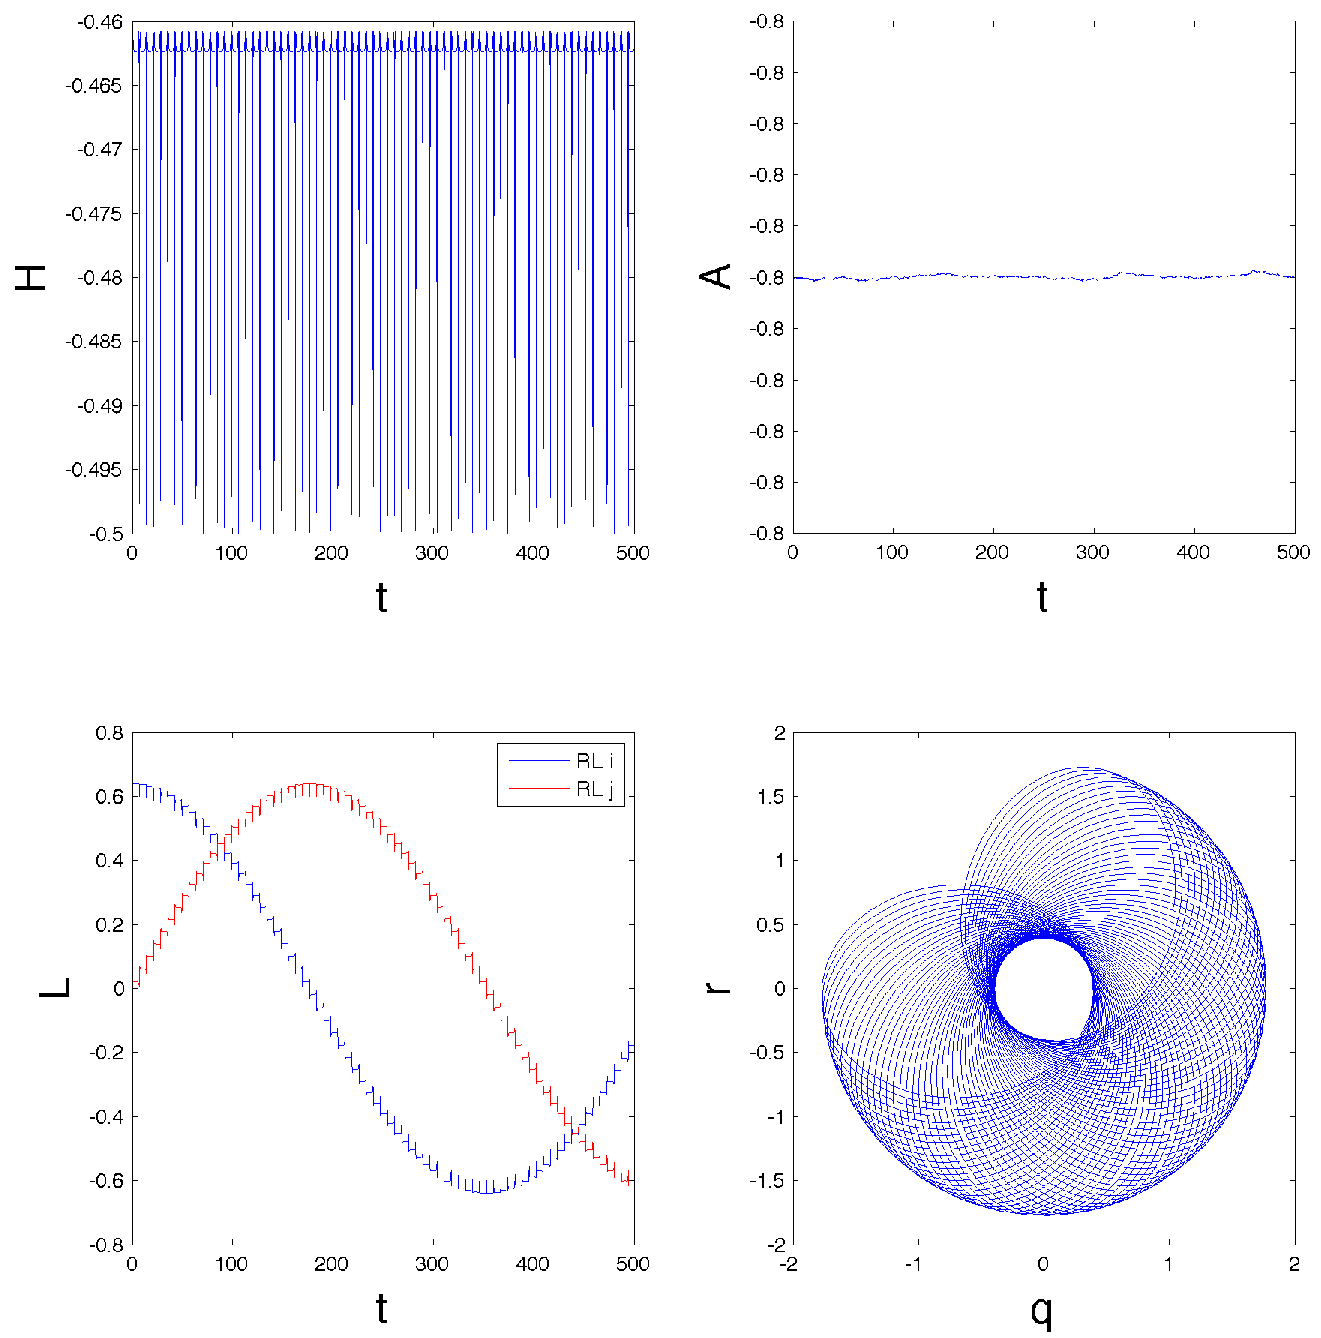
\includegraphics[width=0.5\textwidth]{andy_hw05_prb12_01.pdf}
  \caption{The Kepler two-body problem solved by Verlet-1 with $h = 0.1$. Non conservation of the LRL vector causes the orbit to lose orientation.}
\end{figure}

\begin{figure}[h!]
  \centering
    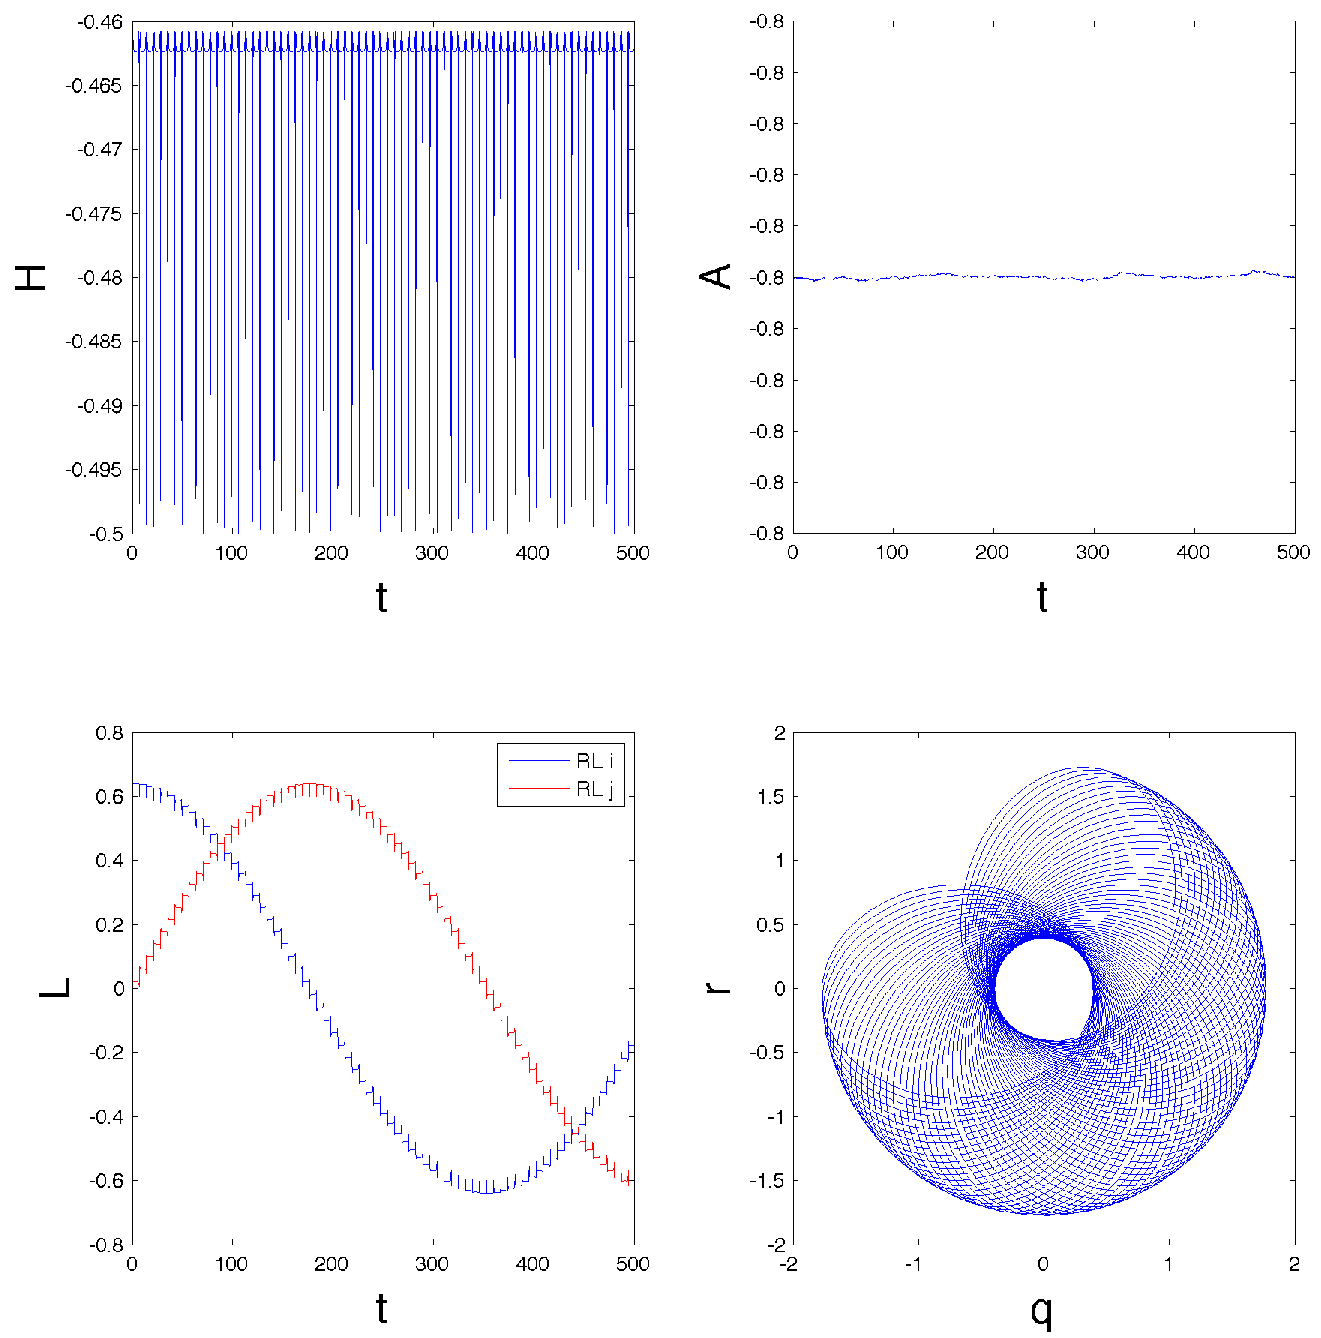
\includegraphics[width=0.5\textwidth]{andy_hw05_prb12_02.pdf}
  \caption{The Kepler two-body problem solved by Verlet-2 with $h = 0.1$. Similarly, non conservation of the LRL vector causes the orbit to lose orientation.}
\end{figure}

\end{enumerate}

%% \begin{figure}[h!]
%%   \centering
%%     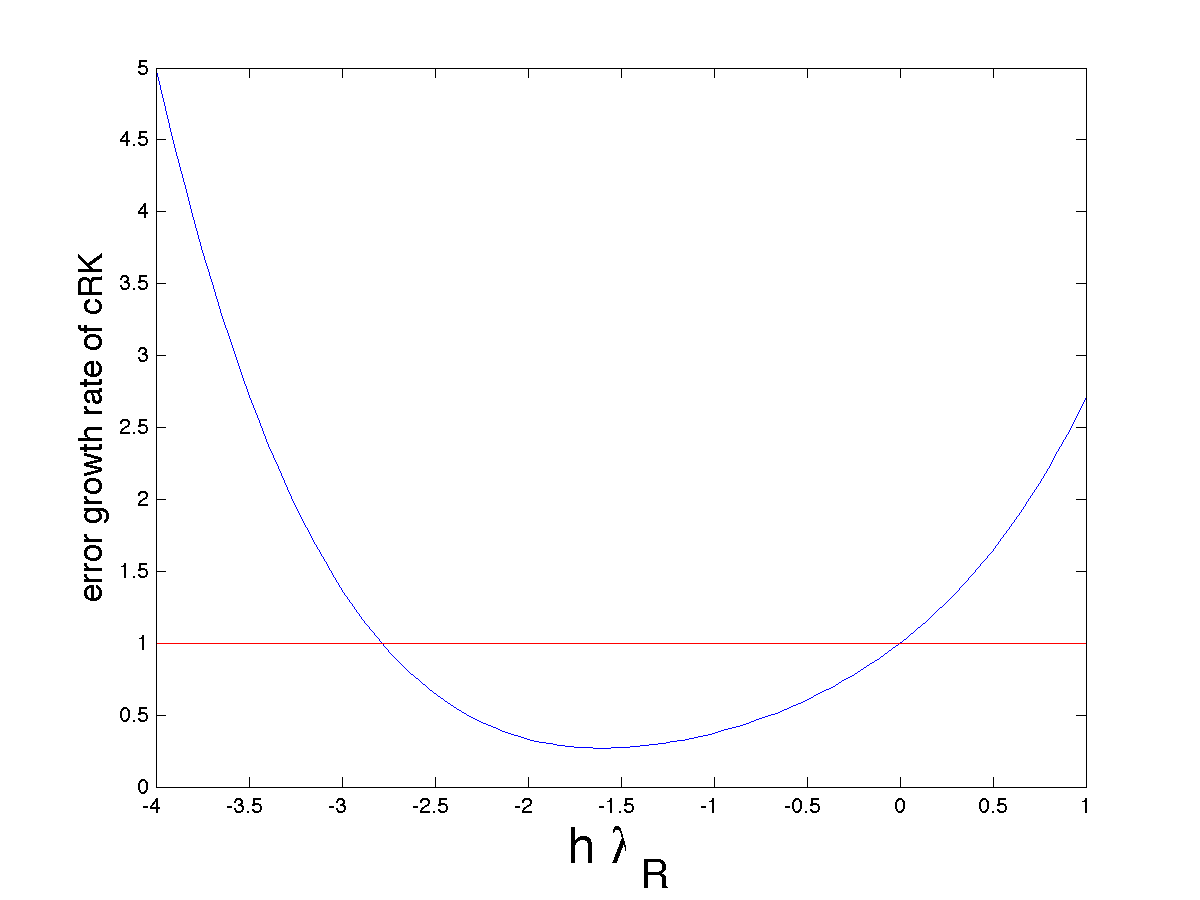
\includegraphics[width=0.5\textwidth]{andy_hw04_prb02_01.png}
%%   \caption{Stability of the cRK method.}
%% \end{figure}

%% \lstinputlisting[language=Matlab]{andy_hw04_prb04.m}

\clearpage
\pagebreak
{\huge Appendix 1: ODE Functions}

\lstinputlisting[language=Matlab]{andy_SHO_1.m}
\lstinputlisting[language=Matlab]{andy_SHO_2.m}
\lstinputlisting[language=Matlab]{andy_SHO_damped.m}
\lstinputlisting[language=Matlab]{andy_kepler2.m}
\lstinputlisting[language=Matlab]{andy_kepler4.m}


\clearpage
\pagebreak
{\huge Appendix 2: Numerical Methods}

\lstinputlisting[language=Matlab]{andy_ME.m}
\lstinputlisting[language=Matlab]{andy_SCD.m}
\lstinputlisting[language=Matlab]{andy_SE.m}
\lstinputlisting[language=Matlab]{andy_cRK.m}
\lstinputlisting[language=Matlab]{andy_symE1.m}
\lstinputlisting[language=Matlab]{andy_symE2.m}
\lstinputlisting[language=Matlab]{andy_symE3.m}
\lstinputlisting[language=Matlab]{andy_verlet1.m}
\lstinputlisting[language=Matlab]{andy_verlet1_2.m}
\lstinputlisting[language=Matlab]{andy_verlet2.m}
\lstinputlisting[language=Matlab]{andy_verlet2_2.m}

\end{document}
